\documentclass{llncs}
\usepackage[ngerman]{babel}
\usepackage[utf8]{inputenc}
\usepackage{listings}
\usepackage{graphicx}
\usepackage{cite}
\usepackage{url}
\usepackage{natbib}



\title{Das Testen von Microservice}
\subtitle{Vorstellung Grundprojekt}
\author{Alexander Piehl\\\email{alexander.piehl@haw-hamburg.de}
\institute{Hamburg University of Applied Sciences (HAW),\\Dept. Computer Science, \\ Berliner Tor 7\\ 20099 Hamburg, Germany\\}}

\begin{document}
\maketitle

\section{Einleitung}
\nocite{*} In der vorliegenden Ausarbeitung wird die erfolgte Arbeit im Grundprojekt zum Entwickeln eines Konzeptes für das Testen von Microservices \cite{fowler2014} dargestellt. Microservice ist eine Architektur, die besonders im Cloud Computing eingesetzt wird. Bei der Architektur wird die gesamte Anwendung vereinfacht gesagt in mehrere kleinere, eigenständige Anwendungen unterteilt. Dies soll mehrere Vorteile bringen wie z.B. bei der Skalierung, der Entwicklung und der Wartung. Durch diese Architektur entstehen aber auch besondere Anforderungen für das Testen. Um auf diese speziellen Anforderungen Lösungen zu finden, soll ein Testkonzept entworfen werden, welches dies übernimmt. Als praktische Anwendungslandschaft dient das an der HAW entwickelte Framework für Multi-Agenten Simulationen MARS.

Das Thema ist aus mehreren Gründen sehr interessant. Zum einen existiert bisher für das Framework MARS keine Teststrategie. Der Aspekt, für diese Anwendung eine eigene Teststrategie zu entwickeln, ist äußerst attraktiv. Verstärkt wird dies noch durch die Verwendung der Microservice-Architektur. Die Architektur ist dabei eine recht neue Architektur, was sie zu einem interessant macht und zum anderen versprechen die Merkmale der Architektur spannende Herausforderungen. Dazu kommt, dass das Framework MARS einen guten Umfang hat. Dies soll heißen, dass es groß genug ist, um aussagekräftige Ergebnisse zu bekommen und es zudem noch übersichtlich genug ist. Ergänzend dazu ist MARS kein künstliches Programm, welches ausschließlich dafür entworfen wurde einen bestimmten Testansatz zu testen. Im Gegenteil ist MARS eine reelle Software, für die es bisher keinen Testansatz existiert.

Dahingehend wird in dieser Ausarbeitung zunächst das Framework MARS vorgestellt und anschließend die Architektur Microservice und den damit verbundenen Vorteilen. Im Anschluss wird im nächsten Kapitel die erfolgte Arbeit im Grundprojekt vorgestellt. Dazu wird in diesem Kapitel auf die einzelnen Arbeitspakete im Grundprojekte eingegangen, wie unter anderem das Ausarbeiten der Herausforderungen und die Implementierung der Testfälle. Im darauffolgenden Kapitel gibt es einen Ausblick auf die Arbeitspakete, welche im Hauptprojekt bearbeitet werden sollen. Diese sind die Entwicklung eines Testkonzeptes für MARS und die vertiefte Arbeit zu den Integrationstest. Zum Schluss wird die erfolgte und die zukünftige Arbeit in einem Fazit zusammengefasst.

\section{MARS \& Microservices}
MARS ist ein Framework für Multi-Agenten Simulationen. Dabei steht MARS für Multi-Agent Research and Simulation und ist ein Forschungsprojekt der HAW Hamburg unter der Leitung von Professor Thiel-Clemen \cite{mars, Huening2016}. MARS bietet Endnutzern die Möglichkeit an über das Framework Multi-Agenten Simulationen durchzuführen. Dabei kann der Endnutzer über die jeweiligen Modelle, die er selber bereitstellen muss, eine spezifische Simulation durchführen lassen. Zurzeit beschränkt sich das Framework auf die Simulation von Öko-Systemen. Daher kann sowohl die Tierwelt in der Savanne ebenso wie in der Arktis simuliert werden. Es müssen nur die entsprechenden Modelle und Daten vorhanden sein.

Das Framework MARS wird als Software as a Service, kurz SaaS, verstanden \cite{Huening2016}. Dies bedeutet, dass die Software und die dazugehörige IT-Infrastruktur dem Endnutzer via API-Schnittstelle und/oder Webseite bereitgestellt wird. Dabei liegen die Software und die IT-Infrastruktur nicht bei dem Endkunden auf einem Computer, sondern bei dem Anbieter der Software oder bei einem externen Dienstleister auf einem Server.

Wie in der Einleitung schon beschrieben, verwendet MARS als Architektur Microservice \cite{Huening2016}.  Microservice ist eine Architektur, die auch von anderen großen Anbietern von SaaS-Plattformen verwendet wird wie z.B. Netflix und Amazon\cite{pattern, heise}. Die Charakteristika von Microservice werden im nächsten Abschnitt näher erläutert.
\subsection{Microservice}
Bei der Microservice Architektur unterteilt sich die Anwendung in mehrere kleinere eigenständige Programme. Im  Kontext der Architektur nennt man die eigenständige Programme Services. Um die Architektur besser zu erläutern, bietet sich die Erklärung von Martin Fowler an. Nach seinem Ansatz lässt sich die Architektur von Microservices am besten im Vergleich mit einer monolithischen Anwendung erklären\cite{fowler2014}. 

\begin{figure}[htbp]
  \centering
      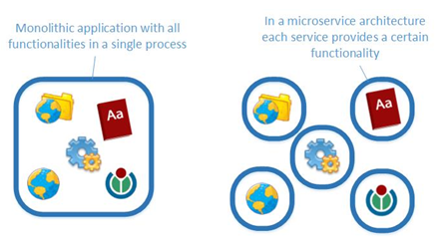
\includegraphics[width=0.7\textwidth]{monolithMicroservice.PNG}
    \caption{Gegenüberstellung monolithische Anwendung und Microservice \cite{locloud}}
    \label{fig:PyramideGoogle}
\end{figure}

Bei einer monolithischen Anwendung befinden sich alle einzelnen Komponenten in einer gemeinsamen großen Anwendung. Am Beispiel MARS wäre in dieser Anwendung unter anderem die Benutzerverwaltung, Projektverwaltung und der Datenimport sowie die GUI enthalten. Bei der Microservice Architektur werden diese Komponenten in eigenständige Programme bzw. Services ausgelagert

Die Erstellung der Services erfolgt nach dem aus der objektorientierten Entwicklung entstandenen Paradigma des Single-Responsibility-Prinzips. Dies bedeutet, dass jeder Service nur eine Aufgabe wahrnimmt, so wie auch ein Objekt nur eine Aufgabe übernimmt. Entweder kümmert sich der Service um die Projektverwaltung oder um die Benutzerverwaltung, aber nicht um beide Tasks gleichzeitig \cite{fowler2014, savchenko2015, savchenko2015microservices}.

Durch die Aufteilung der Aufgaben in einzelnen Services verlagert sich die Komplexität der Software aus dem internen Code-Bereich hinein in die Infrastruktur. Es wird bei Microservice nicht mehr über Klassen, etc. unterteilt welches Objekt bzw. welcher Service welche Aufgabe übernimmt, sondern über einzelne Services. Dahingehend gibt es dafür besondere Anforderungen, die z.B. mit automatisierter Service Deployment, Load Balancing und Continuous Integration gelöst werden sollen \cite{savchenko2015, Fowler2014testing}. 

Von der Architektur verspricht man sich mehrere Vorteile. Aufgrund der Einteilung der Anwendung in mehrere eigenständige Services soll sich die Skalierbarkeit der gesamten Anwendung verbessern. Bei der monolithischen Struktur muss die komplette Anwendung skaliert werden. Bei der Microservice Architektur müssen jedoch nur die Services skaliert werden, bei denen es notwendig ist \cite{fowler2014}. 

Ein weiterer Vorteil betrifft das Deployment. Bei Änderungen an einem Service muss nur dieser Service neu erstellt und veröffentlicht werden. Bei monolithischen Anwendungen muss häufig bei einer Änderung an einer Komponenten die komplette Anwendung neu erstellt und veröffentlicht werden. In der Microservice Architektur betreffen die Änderungen nur den jeweiligen Service, während die anderen Services davon unberührt bleiben und nicht neu erstellt werden müssen \cite{savchenko2015, savchenko2015microservices}. 

Die Microservice Architektur hat auch Auswirkungen auf das Erstellen der Software. Aufgrund der Einteilung der Software in mehrere kleinere Services, welche über HTTP-Schnittstellen wie z.B. REST, JSON kommunizieren, wird eine unabhängigere Entwicklung gefördert. Zum einen gibt es eine klare Aufgabenverteilung, was der einzelne Service leisten muss. Daher ist auch die Aufgabe für die jeweiligen Teams klar definiert. Zum anderen ermöglicht die Kommunikation über HTTP-Schnittstellen, die Services mit unterschiedlichen Programmiersprachen und Technologien zu entwickeln. Dadurch kann für den jeweiligen Service die Programmiersprache und Technologie ausgewählt werden, die am geeignetsten dafür ist \cite{savchenko2015microservices, Ford_2016}.

\section{Grundprojekt}
Die Hauptaufgabe für das Grundprojekt war es eine Grundlage für die weiteren Arbeiten zu schaffen. Dabei wurden für das Grundprojekt vier einzelne Arbeitspakete identifiziert. Diese vier Arbeitspakete waren das Einarbeiten in MARS, der Aufbau einer Testumgebung, das Herausarbeiten der Herausforderungen beim Testen von Microservice und das Erstellen von Systemtest bzw. GUI-Tests mit dem Framework Selenium. Zusätzlich erfolgten Recherchen für das nachfolgende Hauptprojekt.

Das erste Arbeitspaket ist in dem Sinne selbsterklärend, dass es ohne Einarbeitung in MARS schwierig ist, die Herausforderungen für das Testen herauszuarbeiten und erste Testfälle dafür zu konzipieren. Dabei konzentrierte sich die Einarbeitung zunächst darauf die Bedienung der Weboberfläche zu verstehen, damit die notwendigen Schritte bekannt sind, wie eine Simulation via MARS ausgeführt wird. Auf diese Einarbeitung erfolgte eine erste Analyse der Architektur sowie der Implementierung, soweit es für das Grundprojekt notwendig war. Diese Analyse soll im Hautprojekt vertieft werden.

\subsection{Aufbau der Testumgebung}
Im zweiten Arbeitspaket wurde eine Testumgebung für MARS aufgebaut. Wie schon in der obigen Einleitung kurz beschrieben, wurde nur die Weboberfläche getestet. Dahingehend beschränkt sich das Testen in diesem Projekt alleine auf die Webschnittstelle und deren Aufrufung durch den Client bzw. durch die Webseite. Auf Grundlage dessen ist auch die Testumgebung konstruiert. Für die Testumgebung wurde eine Virtuelle Maschine, im weiteren mit VM abgekürzt, erstellt, auf welcher die Linux Distribution Ubuntu installiert worden ist. Auf dieser VM wurde eine lokale MARS-Version installiert.

Für die lokale MARS-Installation gibt es kein Installationsprogramm oder Ähnliches. Die Installation erfolgte über eine interne Anleitung der MARS-Gruppe. Dafür wurde der Source Code aus einem Git Repository ausgecheckt. Dementsprechend musste GIT installiert sein. Ergänzend dazu müssen die Programme Docker sowie Docker Compose installiert werden. Sobald die Installation erfolgreich verlaufen ist, kann die lokale MARS Version über einen Browser unter der Localhost Adresse aufgerufen werden. 

Im Anschluss wurden auf der VM noch die aktuellste Eclipse Version geladen, um mit Eclipse die Systemtests zu implementieren. Zusätzlich mussten noch das Framework Selenium geladen werden und die Jar-Dateien in Eclipse als Library eingebunden werden, damit das Framework verwendet werden kann. Dazu wurde vom aktuellen Entwicklungszweig ein Branch erstellt. Auf diesem Branch wurden keine Änderungen eingepflegt, sondern nur die erstellten Systemtests hinzugefügt. Daher wurde mit einer eingefrorenen MARS-Version gearbeitet.

Für die Erstellung der Systemtests wurde zudem noch Testdaten benötigt. Besonders für das Testen des Imports wurden Test-Dateien benötigt. Diese wurden von der MARS-Forschungsgruppe bereitgestellt. Dabei handelte es sich um Modelle und Dateien in bestimmten Formaten, welche für eine Simulation notwendig sein können. Namen von Projekten und ähnliches wurden freigewählt.

\subsection{Herausforderungen an das Testen}
Im dritten Arbeitspaket wurden die Herausforderungen, die durch die Architektur und dem aktuellen Status des MARS Frameworks herausgearbeitet. In diesem Kapitel werden nicht ausschließlich die allgemeinen Herausforderungen vorgestellt, sondern auch jene, die spezifisch für MARS sind. MARS ist in einem sehr fortgeschrittenen Status und befindet sich kurz vor dem ersten offiziellen Release. Dies bedeutet, dass das Testen nicht von Anfang an Bestandteil der Implementierung war, sondern in einen bestehenden Prozess integriert werden muss. Im Detail bedeutet das, dass kein iterativer Aufbau des Systems begleitet wird, sondern mit einem bestehenden System gearbeitet wird, welches laufend Änderungen erhält. Dies ist für eine Microservice-Anwendung nichts ungewöhnliches, da es gerade wegen der Architektur möglich ist das System laufend zu verändern. Jedoch muss dafür ein Testansatz gefunden werden, welcher darauf flexibler reagiert. Der Testansatz sollte so flexibel sein, dass Änderungen an der Anwendung nicht zur erheblichen Mehrarbeit bei der Aktualisierung der Tests führt.

Die nächsten beiden Herausforderungen liegen recht nah beieinander und zwar die Möglichkeit des schnellen Wechseln der Komponenten sowie der häufigen Releases. Dies sind beides Vorteile der Microservice Architektur. Da die Services schnell gewechselt werden können und dadurch häufiger veröffentlicht werden können, benötigt man ein Testkonzept, welches darauf optimiert ist. Einerseits müssen die jeweiligen Tests so gründlich sein, dass der Service als Einzelkomponente funktioniert und in der Zusammenarbeit mit den anderen Services keine Fehler entstehen. Dabei werden verschiedene Testebenen angesprochen. Beim Testen der Services spielen sowohl Unit-Tests, Integrationstests und Systemtests eine Rolle. Ein Service besteht aus mehr als einer Funktion bzw. Klasse. Auch hier gibt es verschiedene Klassen und Methoden, welche zusammenarbeiten. Dahingehend sollten die einzelnen Funktionen mit Unit-Test bedacht werden. Neben dem Zusammenwirken von verschiedenen Klassen im Service, können sie auch eigene externe Komponenten wie Datenbank besitzen. Daher sollten auch diese Verbindungen auf der Ebene der Integrationstest getestet werden. Schlussendlich muss auch der Service als ein zusammenhängendes System getestet werden, um zu prüfen, ob er seine Anforderungen erfüllt. Erst danach könnte das Zusammenwirken der einzelnen Services getestet werden, was wiederum auch der Ebene der Integrationstests entsprechen würde, aber auf das Gesamtsystem bezogen.
Neben dem gründlichen und ausführlichen Testen benötigt man jedoch auch ein schnelles Feedback von den Tests. Ein großer Vorteil der Architektur liegt gerade im schnellen Austausch der Services und den damit verbundenen häufigen Releases. Allerdings geht dieser Vorteil verloren, wenn sich der Test für einen Service über mehrere Stunden zieht. Diese Vorteile bleiben nur bei einem effizienten Testkonzept erhalten. Zusammengefasst müssen die Tests gründlich sein und gleichzeitig ein schnelles Feedback geben, um diese Herausforderungen zu meistern.

Die nächste Herausforderung ist das unabhängige Entwickeln der Services. Besonders die Verwendung von unterschiedlichen Programmiersprachen und Technologie müssen beim Testkonzept beachtet werden. Da jede Technologie ihre Stärken und Schwächen hat, muss das Testen darauf reagieren und sich teilweise auf unterschiedliche Aspekte gleichzeitig konzentrieren. Dazu gehören auch die Herausforderungen, die durch das unabhängige Austauschen der Microservices vorhanden sind. Die einzelnen Services sind wie oben genannt eigenständige kleinere Anwendungen, die über HTTP-Schnittstellen kommunizieren. Daraus folgt, dass die HTTP-Schnittstellen eine sehr wichtige Aufgabe übernehmen. Daher müssen diese HTTP-Schnittstellen ausführlich getestet werden. Dazu kommt die Situation, dass dem Tester bzw. dem Test nicht bekannt ist, dass von einem anderem Service eine neuere Version vorliegt. Auf solche Umstände muss das Testkonzept auch eingehen können.

Bei Microservice müssen nicht nur selbst entwickelte Services verwendet werden, sondern es können auch Services von Dritten verwendet werden. Bei der Verwendung von externen Services kann es immer wieder sein, dass über den Service Informationen fehlen. Es ist nicht unüblich, dass bei einem externen Service nur die Schnittstelle bekannt ist. Dies mag für die Nutzung auf den ersten Blick zu keinen Problemen führen, aber beim Testen kann dies schon zu ersten Schwierigkeiten führen. Aufgrund fehlender Informationen können die Tests gegebenenfalls nicht optimal erstellt werden.

Die oben ausgeführten Herausforderungen sind keine unbekannten Probleme. Da Microservices auf Grundlage von Service Oriented Architecure(SOA) entstanden bzw. eine Weiterentwicklung davon ist, gibt es diese ähnlichen Herausforderungen auch bei Service Oriented Architecure. Auch bei der komponentenbasierten Entwicklung, welche Microservice sehr ähnlich ist, gibt es diese vergleichbaren Herausforderungen. Dies hat zur Folge, dass man ggf. auf ähnliche Arbeiten in diesem Bereich zurückgreifen kann\cite{savchenko2015}.

\subsubsection{MARS spezifische Herausforderungen}
Einige der von MARS implementierten Services werden erst bei der Durchführung der Simulation aufgerufen. Zwar ist zurzeit definiert nur die vorbereitenden Schritte für die Ausführung einer Simulation zu testen. Jedoch sollte man sich auch Gedanken darüber machen, wie man die Services testen kann, welche nur bei der Durchführung der Simulation aufgerufen werden. Die Herausforderung ist dabei, diese Services zu testen ohne eine Simulation zu starten, was einen sehr großen Aufwand bedeuten würde. Es muss eine Lösung gefunden werden, wie man aussagekräftige Tests implementieren kann, ohne den Aufwand einer Simulation zu haben.

Des Weiteren besteht die Herausforderungen, dass für MARS keine Anforderungen oder User Stories definiert sind. Daher ist es kompliziert Testfälle zu generieren. Dies trifft besonders auf die Erstellung der Systemtests für das Gesamtsystem bzw. der Oberfläche  zu, da dieser per Definition aus den Anforderungen erstellt werden soll. Interessant an dieser Stelle ist zu prüfen, ob  Error Guessing \cite{homes2013fundamentals} und/oder Exploratory Testing \cite{bach2003exploratory} unterstützend wirken können, um die Testfälle zu erstellen. Bei der Verfahrensweise Error Guessing geht es darum, aufgrund von Erfahrungen und Kenntnisse über das Programm mögliche Fehler zu erraten und diese mit den Testfällen zu entdecken. Exploratory Testing wird häufig missverstanden als einfaches 'durchklicken' einer Anwendung. Bei Exploratory Testing versucht der Anwender jedoch durch aktives Steuern bzw. Testen der Anwendung neue Informationen über die Anwendung zu sammeln und daraus neue Testfälle zu generieren. 

\subsection{Systemtests MARS}
Das vierte Arbeitspaket im Grundprojekt war die Erstellung von Systemtests von MARS und deren Umsetzung. In der Tabelle 1 sind die fünf Testfälle beschrieben, welche für die MARS Oberfläche entworfen worden sind. Dabei werden die einzelnen Schritte durchgegangen, welche man für das Starten einer Simulation benötigt. Der Anwender/Tester muss sich zunächst in der Web-Oberfläche anmelden. Nach der Anmeldung soll ein neues Projekt erstellt und anschließend auch ausgewählt werden. Nach der Auswahl des Projektes können die benötigten Daten und Modelle in unterschiedlichen Schritten importiert werden. Danach könnte die Simulation gestartet werden. Dies wird jedoch nicht gemacht, weil es zu einem die virtuelle Maschine nicht leisten kann und zum anderen nicht Bestandteil meiner Tests ist. 
\subsubsection{Beschreibung der Testfälle}

Aus dem oben beschriebenen generellen Ablauf, können die fünf folgende Testfälle beschrieben werden:
\begin{table}[]
\centering
\label{MARS_Testfaelle}
\begin{tabular}{|c|l|p{4cm}|p{4cm}|}
\hline
\multicolumn{1}{|l|}{Nummer} & Name              & Beschreibung & Erwartetes Ergebnis \\ \hline
1 & Anmelden          & Eingabe der Anmeldedaten in die Anmeldemaske & Man konte sich mit den Daten Anmelden und die Projektübersichtsseite wird angezeigt \\ \hline
2 & Projekt erstellen & Erstellung eines neuen Projektes & Projekt wurde erstellt und erscheint in der Übersicht der Projekte \\ \hline
3 & Projekt auswählen & Das eben erstellte Projekt als aktuelles Projekt auswählen & Meldung erscheint, dass das Projekt ausgewählt worden ist  \\ \hline
4 & Daten importieren & Die für die Simulation benötigten Daten müssen importiert werden & Es wurden die richtigen Daten ausgewählt und erfolgreich importiert  \\ \hline
5 & Modelle laden     & Die Modelle für die Simulation müssen geladen werden & Die Modelle wurden erfolgreich geladen \\ \hline
\end{tabular}
\caption{MARS Testfälle}
\end{table}

\subsubsection{Testfall 1: Anmelden}
Wie in der Tabelle 1 beschrieben, wird in diesem Testfall das Anmelden getestet. Dafür werden die Anmeldedaten eingegeben, um zu prüfen, ob die Anmeldung erfolgreich war. Zurzeit befindet sich diese Funktion noch in einer Beta-Phase. Die vorhandenen Anmeldedaten wie Name, E-Mail und Passwort befinden sich zurzeit noch unverschlüsselt in einer Text-Datei. Das Anmelden wird ausschließlich mit gültigen Anmeldedaten getestet. Das Verhalten bei falschem Benutzername und/oder Passwort wird nicht getestet. Denn zum Zeitpunkt des Testens war das Verhalten für falsche Benutzereingaben noch nicht implementiert. Jedoch wurden die Tests dafür schon implementiert.

Ob die Anmeldung erfolgreich war, wird anhand der URL überprüft. Beim Anmelden lautet die URL "http://localhost/login". Nach einer erfolgreichen Anmeldung ändert sich die URL zu "http://localhost/". Auf diese Veränderung hin wie die URL wird untersucht. 

Darauf folgend wird noch überprüft, ob die richtige Seite aufgerufen wird. Sollte die erste Prüfung mit der URL erfolgreich sein, wird kontrolliert ob die Seite mit der Übersicht der Projekte angezeigt wird. Dafür wird getestet, ob an der entsprechenden Stelle der Text 'Your Projects' steht. Ist diese Prüfung korrekt sowie die Prüfung auf die Veränderung der URL, gilt der Testfall als bestanden.

\subsubsection{Testfall 2: Projekt erstellen}
Im zweiten Testfall geht es darum zu prüfen, ob die Erstellung von Projekten korrekt funktioniert. Für diesen Testfall wird ein neues Projekt angelegt. Jedes Projekt benötigt einen eindeutigen Namen. Dazu können optional eine Projektbeschreibung und Tags zum Projekt mit angegeben werden. In diesem Testfall wird neben dem Name auch eine Beschreibung des Projektes sowie mehrere Tags eingegeben. Sollte das Projekt korrekt angelegt worden sein, wird das neue erstellte Projekt in einer Übersichtsseite für die Verwaltung der Projekte angezeigt. Zur abschließenden Kontrolle wird nun auf dieser Projekt Übersichtsseite versucht den Namen, die Beschreibung und die Tags des Projektes auszulesen. Wenn dies funktioniert und die ausgelesenen Texte die selben sind wie die eingegebenen Texte, gilt der Test als bestanden.

\subsubsection{Testfall 3: Projekt auswählen}
Der dritte Testfall ist ein relativ kleiner Testfall. Bei diesem Test geht es nur darum, zu prüfen, ob nach der Erstellung des Projektes auch dieses ausgewählt werden kann. Dafür wird die Startseite bzw. die Projekt Übersichtsseite geladen. Diese Seite wird auch nach der erfolgreichen Anmeldung angezeigt. Auf dieser Seite wird nun versucht das Projekt auszuwählen. Sobald das Projekt ausgewählt worden ist, wird eine Meldung angezeigt. Der Text aus dieser Meldung wird ausgelesen und mit einem Soll-Text verglichen. Der Soll-Text wurde von der MARS-Gruppe definiert. Bei Gleichheit der Texte gilt der Testfall als bestanden.

\subsubsection{Testfall 4: Daten importieren}
Nachdem das Projekt erfolgreich ausgewählt wurde, müssen nun die notwendigen Daten importiert werden. Um die Daten importieren zu können, muss zunächst die dafür zuständige Unterseite geladen werden.
Der Import der Daten ist in drei Schritten unterteilt. Im ersten Schritt muss eine Datei, z.B. eine CSV-Datei, ausgewählt werden, welche importiert werden soll. Diese Dateien beinhaltet z.B: Informationen über Populationen eines bestimmten Tieres. Diese Informationen sind für die Simulation notwendig. Im nächsten Schritt müssen die importierten Daten genauer spezifiziert werden. Dies kann entweder darüber geschehen, dass man die Autorin bzw. die Autoren der Daten angibt oder die Organisation benennt. Beim darauffolgenden und letzten Schritt müssen die Daten einer Kategorie zugeordnet werden. Dazu kann eine bestehende Kategorie ausgewählt werden oder eine neue Kategorie erstellt werden. Die Kategorien können freigewählt werden und beliebig erweitert werden. Die Kategorien sollen die importierten Daten genauer spezifizieren, um unter anderem die Suche nach bestimmten Daten zu erleichtern.
Im Testfall 4 werden diese einzelnen Schritte ausgeführt. Zunächst wird eine CSV-Datei importiert und im Anschluss wird für diese Daten ein Autor angegeben. Danach wird eine neue Kategorie erstellt und den importierten Daten zugeordnet. Nachdem all diese Schritte ordnungsgemäß durchgeführt worden sind, ist der Button für den Import auswählbar. Daraufhin wird eine neue Seite angezeigt, bei der der Fortschritt des Imports angezeigt wird. Sobald das Textfeld nicht mehr den Text 'Running' anzeigt, wird kontrolliert, ob nun im Textfeld 'Finish' steht. Ist dies der Fall, gilt der Testfall als bestanden.

\subsubsection{Testfall 5: Modelle laden}
Im letzten Testfall wird das Laden der Modelle getestet. Um ein Modell für die Simulation zu laden, muss zunächst ein Modell ausgewählt werden. Diesem Modell muss ein eindeutiger Name zugeordnet werden. Dazu kann man dem Modell auch eine Beschreibung hinzufügen.
Es wird bei diesem Testfall ein Modell ausgewählt und zudem Name sowie Beschreibung hinzugefügt. Nachdem der Button für Laden des Modells gedrückt wurde, muss noch eine Meldung bestätigt werden. Erst nach der Bestätigung der Meldung wird das Modell geladen. Im Anschluss darauf wird nun geprüft, ob der Name des Modells in der Übersicht der geladenen Modelle auftaucht. Sollte dies der Fall sein, gilt auch dieser Test als bestanden.

Mit dem Abschluss der fünf Testfälle wurde der Hauptpfad in der MARS-Oberfläche getestet. Mit diesen Testfällen sind die einzelnen Schritte abgedeckt, die mindestens benötigt werden, um eine Simulation durchzuführen.

\subsection{Testabdeckung}
In der Tabelle 2 ist dargestellt, welche Microservices durch die Testfälle abgedeckt werden und welche nicht. Erwähnt werden muss dabei, dass zurzeit bei MARS eine große Umstellung stattfindet, welche besonders die Weboberfläche betrifft. Das Frontend war ursprünglich ein Service. Jedoch wird das Frontend zurzeit in mehrere Microservices unterteilt. Daher befinden sich noch einige Microservices in der Implementierung. Die in der Tabelle 2 dargestellten Microservices sind die, wie sie nach der Umstellung vorhanden sein sollen. Teilweise werden die neuen Microservices nach ihrer Implementierung von den vorhandenen Testfällen schon abgedeckt, wie z.B. der Service UserLoginService. Daher gelten diese Microservices auch als abgedeckt.

Es werden ungefähr die Hälfte der Microservices mit den Testfällen abgedeckt. Die meisten Microservices, welche zurzeit nicht abgedeckt werden, werden erst verwendet, wenn die Simulation gestartet wird. Da nur die vorbereiteten Schritte für die Simulation in den Testfällen abgebildet werden, können diese Microservices durch die bisherigen Testfälle auch nicht abgedeckt werden.

Der Service für den GISImport ist nicht abgedeckt, weil beim Laden der Modelle ein anderes Format als das GIS-Format gewählt wird. Dementsprechend kann man den Testfall 5 anpassen, damit auch dieser Service mit abgedeckt ist.

\begin{table}[]
\centering
\label{MARS_Abdeckung_Services}
\begin{tabular}{|c|l|p{4cm}|p{4cm}|}
\hline
\multicolumn{1}{|l|} {Name} & abgedeckt & Testfall \\ \hline
FrontEnd & ja &  Alle Testfälle \\ \hline
Zuul & ja & Alle Testfälle \\ \hline
Eureka & ja & Alle Testfälle \\ \hline
ConfigService & ja &  Alle Testfälle \\ \hline
UserLoginServcie & ja & Testfall 1\\ \hline
AccessTokenService & ja & Testfall 1\\ \hline
FileService  & ja & Testfälle 4 \& 5 \\ \hline
TableBasedImport & ja & Testfall 4\\ \hline
TimeSeriesImport & ja & Testfall 4 \\ \hline
ModelImport & ja & Testfall 5 \\ \hline
MetaDataService & ja & Testfall 5\\ \hline
GISImport & nein & \\  \hline
DataValidation & ja & Testfälle 4 \& 5 \\ \hline
DataPreview & ja & Testfälle 4 \& 5 \\ \hline
ReflectorService & nein & \\ \hline
ShuttleFileService & nein & \\ \hline
ShuttleInterpretor & nein & \\ \hline
DockerService & nein & \\ \hline
SimControlService & nein & \\ \hline
PerfomanceService & nein & \\ \hline
SimulationManager & nein & \\ \hline
LayerContainer & nein & \\ \hline
ResultConfigService & nein & \\ \hline
VisualAnalytics & nein & \\ \hline
UnityVisuzalization & nein & \\ \hline
VisualizationService & nein & \\ \hline
\end{tabular}
\caption{Abdeckung der Microservices}
\end{table}

\subsection{Umsetzung der Testfälle}
Die oben fünf beschriebenen Testfälle wurden alle mit Selenium in Verbindung mit dem Framework JUnit erstellt. Selenium ist eine Anwendung für die automatisierte Durchführung Tests von Web-Anwendungen \cite{selenium}. Dafür können in Selenium Skripte definiert werden, die eine Interaktion mit einer Webseite simulieren bzw. durchführen. Mit den selbst definierten Skripten können die Interaktionen wiederholt und automatisch durchgeführt werden. Dahingehend eignet sich Selenium sehr gut für GUI-Tests bei Webseiten und auch für Regressionstests bei Webseiten \cite{selenium}. 

Das Selenium Framework bietet mehrere unterschiedliche Komponenten an. Das Framework selbst unterscheidet zwischen dem Selenium WebDriver und der Selenium IDE. Laut Homepage von Selenium sei der WebDriver dafür gedacht robuste und browser-basierte Testfälle und Testsuites zu erstellen \cite{selenium}.  Dabei sei dieser für automatische Regressionstest geeignet. Dazu seien die Skripts verteilbar und skalierbar über mehrere Umgebungen hinweg. Die Selenium IDE hingegen sei für schnelle Bug-Tests geeignet und hätte zudem das Ziel, automatisches exploratory testing durchzuführen \cite{selenium}. 

Für diesen Anwendungsfall eignet sich am besten der Selenium WebDriver, da es erstens darum geht automatische Regressiostest zu erstellen, da nach jeder Änderungen an einem Service geprüft werden soll, ob die generelle Funktionalität noch vorhanden ist. Zum zweiten sollen die Testfälle langfristig mit mehreren unterschiedlichen Browsern getestet werden.

Für die Verwendung des Selenium WebDrivers wird ein lokaler Selenium Client benötigt. Die Skripts für den WebDriver und den Client können in verschiedenen Sprachen bzw. Skriptsprachen angelegt werden. Dabei unterstützt das Selenium Framework folgende Sprachen: Java, C\#, Ruby, Python und Javascript(Node). Es stehen noch mehr mögliche Sprachen zur Verfügung, welche aber nicht vom Selenium Hauptprojekt unterstützt werden, sondern von unabhängigen Dritt-Entwicklern bereitgestellt werden. Für die Erstellung der Skripts wurde die Programmiersprache Java verwendet, da mit dieser Programmiersprache die größte Erfahrung vorlag. 

Wie schon oben erwähnt werden die Testfälle via Selenium browser-spezifisch erstellt. Dies bedeutet, dass für die einzelnen Browser wie Firefox, Chrome und Internet Explorer eigene WebDriver zur Verfügung stehen. Zunächst wurden die Testfälle nur für den Firefox-Browser erstellt. Dies hat mehrere einfache Gründe. Der Firefox Browser verfügt über gute Entwicklungstools, die für die Erstellung der Testfälle notwendig sind. Dazu sind viele Tutorials zu Selenium in Verbindung mit dem Firefox-Browser zur weiterführenden Recherche verfügbar.

\subsubsection{Grundlagen Selenium}
Der erste Schritt beim Schreiben des Skriptes für die Interaktionen mit der Webseite, ist das Erstellen eines WebDriver-Objektes. Das WebDriver-Objekt ist die Grundlage dafür, die einzelnen Interaktionen durchzuführen.

\lstset{language = Java}
\begin{lstlisting}
 public WebDriver createDriver(){
		WebDriver driver = new FirefoxDriver();
		driver.navigate().to("http://localhost/login");
		
		return driver;
	}
\end{lstlisting}

Wie in der obigen Code-Zeile dargestellt, wird ein WebDriver-Objekt für den Firefox-Browser erstellt. An dieser Stelle wird unterschieden, für welchen Browser der WebDriver gedacht ist. Mit dem erstellten WebDriver können die Interaktionen durchgeführt werden. Als ersten Schritt muss die Website aufgerufen werden. Dies geschieht mit den Methoden vom WebDriver-Objekt: "driver.navigate().to();". In der Methode "to()" wird die Adresse der Webseite, in diesem Fall "http://localhost/login", als Argument übergeben. Damit wird die Anmeldeseite von MARS aufgerufen. 


\lstset{language = Java}
\begin{lstlisting}
public String[] login(WebDriver driver, String email, String password){
	driver.findElement(By.id("email")).sendKeys(email);
	driver.findElement(By.id("password")).sendKeys(password);
	driver.findElement(By.
	xpath(".//*[@id='loginForm']/div[2]/button[3]")).click();
		
	WebDriverWait wait = new WebDriverWait(driver, 10);
	WebElement element = wait.
	until(ExpectedConditions.
	elementToBeClickable(By.
	xpath(".//*[@id='content']/div/div[1]/div[1]/div/div/a")));
		
	String [] result = new String[2];
		
	result[0] = driver.getCurrentUrl();
	System.out.println("CurUrl: " + result[0]);
	if(result[0].equals("http://localhost/")){
		result[1] = driver.
		findElement(By.
		xpath(".//*[@id='content']/div/div[1]/div[1]/div/h3")).
		getText();
	}else {
		result[1] = driver.
		findElement(By.
		xpath(".//*[@id='loginForm']/div[1]/p[2]")).getText();
	}
		
	return result;
}
\end{lstlisting}

Nachdem die Anmeldeseite aufgerufen worden ist, folgt die oben dargestellte Methode. Diese Methode hat die Aufgabe die Anmeldedaten in die entsprechenden Felder einzugeben und sich im Anschluss anzumelden. Diese Methode soll als ein generelles Beispiel dienen, wie die Interaktionen mit der Webseite über Selenium laufen. Wie oben bereits beschrieben, laufen die Interaktionen mit der Webseite über das WebDriver-Objekt. Mit die wichtigste Methode vom WebDriver-Objekt ist die Methode "findElement()". Die Methode hat die Aufgabe, das Element zu finden mit dem interagiert werden soll. Dabei kann das Element ein Button, ein Textfeld oder ähnliches sein. Um das Element zu finden bekommt die Methode als Argument einen Selektor übergeben, worüber das Element gefunden werden kann.  Das gesuchte Element kann über verschiedene Wege gesucht werden. Wie im obigen Beispiel kann das Element über seine ID gefunden werden. Dies funktioniert aber nur, wenn das Objekt eine eindeutige ID im HTML-Code bekommen hat. Dazu bestehen noch die Möglichkeiten Elemente über ihren Klassennamen oder über den CSS-Selektor zu finden. Sollte das Element über diese Möglichkeiten nicht gefunden werden können, kann das Element auch über den sogenannten XPath gefunden werden. Der XPath ist eine vom W3-Konsortium entwickelte Abfragesprache für XML-Dateien, um diese auslesen zu können.

Der XPath kann im Gegensatz zur ID nicht einfach aus dem Quellcode ausgelesen werden. Dafür empfiehlt sich, auch bei dem Bestimmen der ID, auf Browser interne Entwicklertools zurück zugreifen. Fast alle Browser bieten Entwicklungstools wie den Inspektor an. Mit diesem Inspektor können bestimmte Elemente ausgewählt werden und der Browser zeigt die dazu gehörige Stelle im HTML-Code an, wo man die ID oder den XPath auslesen kann.

Sobald das Element gefunden ist, können Interaktionen mit dem Element durchgeführt werden. Die Interaktionen können dabei unterschiedlich sein und sind teilweise auch abhängig vom vorliegenden Element. Buttons können mit der Methode click() ausgeführt werden. Um Text einzugeben, wird die Methode sendKeys() verwendet. Wie in der obigen Methode dargestellt, wird damit jeweils die E-Mail Adresse und das Passwort darüber eingegeben. Der jeweilige Text wird als String der Methode als Argument übergeben. 

Nachdem die Anmeldedaten eingeben wurden sind, wird der Anmelde-Button ausgeführt. Ob das Anmelden erfolgreich war, wird daran geprüft, ob sich die URL geändert hat. Da es einige Zeit dauern kann, bis die Abfrage für das Anmelden bearbeitet wurde und sich damit auch die URL ändert, wird zunächst mit Hilfe des WebDriverWait-Objektes gewartet. Dabei wird geprüft, ob ein bestimmtes Element auf der Seite nach der Anmeldung anwählbar ist. Dabei wird bis zu 10 Sekunden gewartet, ob das Element anwählbar ist. Sollte es nach zehn Sekunden immer noch nicht anwählbar sein, wird Selenium eine Exception werfen.

Anschließend wird die URL mit dem Befehl driver.getCurrentURL() ausgelesen. Zunächst wird überprüft, ob die URL mit der Soll-URL übereinstimmt, welche nach der Anmeldung vorhanden sein sollte. Ist diese Überprüfung korrekt, wird kontrolliert, dass die richtige Seite geladen wurden ist. Dafür wird wieder ein bestimmtes Element ausgewählt und der Text vom Element ausgelesen. Dies geschieht mit der Methode getText(). 

Wenn die URL nicht mit der Soll-URL übereinstimmt, wird davon ausgegangen, dass die Anmeldung nicht erfolgreich war. Daraufhin wird die Meldung ausgelesen, die angibt, warum die Anmeldung nicht erfolgreich war. Dieser Fall ist für diesen Testfall unbedeutend, da nur geprüft werden soll, ob mit korrekten Anmeldedaten die Anmeldung funktioniert. Der Fall dient ausschließlich für spätere Erweiterungen. Damit geprüft werden kann, dass die angezeigten Fehlermeldung den richtigen Grund für die fehlgeschlagene Anmeldung anzeigt, wie z.B. E-Mail-Adresse nicht gefunden.

\subsubsection{Prüfung der Ergebnisse mit JUnit}
Die von der Methode zurückgegebenen Werte werden anschließend mit JUnit überprüft. JUnit ist ein Testing Framework und eigentlich für Unit-Tests gedacht, wie der Name schon vermuten lässt. Mithilfe von JUnit können die Tests automatisiert gestartet werden und am Ende der Tests wird eine Übersicht erstellt, die zeigt welche Tests erfolgreich waren und welche fehlgeschlagen sind.

\lstset{language = Java}
\begin{lstlisting}
@Test
public void testHappyPath(){
	LogIn logIn = new LogIn();
	Projects projects = new Projects();
	ImportData importData = new ImportData();
	Models models = new Models();
		
	String[] resLogin = logIn.logIn(driver);
	String[] resCreateProjects = projects.createProject(driver);
	String resChooseProjects = projects.chooseProject(driver);
	String resImportData = importData.toImportData(driver);
	String resModels = models.LoadModel(driver);
		
	assertEquals(resLogin[0],"http://localhost/");	
	assertEquals(resLogin[1],"Your Projects");	
		
	assertEquals(resCreateProjects[0],"Test Projekt");
	assertEquals(resCreateProjects[1],"Dies ist ein Test Projekt");	
	assertEquals(resCreateProjects[2],"Test, Selenium, Projekt");	
		
	assertEquals(resChooseProjects,"Project \"Test Projekt\" selected.");
		
	assertEquals(resImportData,"Finished");
		
	assertEquals(resModels,"KNP_Model");
	}
\end{lstlisting}

Da die einzelnen Testfälle alle hintereinander ablaufen müssen, befinden sich alle Testfälle in einer Test-Methode von JUnit. Bei mehreren einzelnen Test-Methoden von JUnit kann die Reihenfolge nicht festgelegt werden und der Aufruf der einzelnen Test-Methoden erfolgt nicht-deterministisch.

Daher werden in dieser Methode alle Testfälle aufgerufen, damit die Reihenfolge bestimmt werden kann. Für das Überprüfen der Ergebnisse wird die Methode assertEquals() von JUNit verwendet. Die bekommt als erstes Argument den IST-Wert und als zweites den SOLL-Wert übergeben. Wenn beide Werte übereinstimmen gilt der Testfall als erfolgreich.

\subsection{Recherche Teststrategien}
Als Vorbereitung für das nachfolgende Hauptprojekt wurde nach Teststrategien gesucht, welche sich für eine Microservice-Anwendung eignen könnten. Dabei wurden zwei verschiedenen Ansätze gefunden. Der erste Ansatz ist die von Martin Fowler entworfene Teststrategie für Microservices \cite|{Fowler2014testing}. Der zweite Ansatz ist die von Google entwickelte Teststrategie \cite|{whittaker2012google}. In den nächsten beiden Abschnitten werden die einzelnen Ansätze ausführlicher vorgestellt.

\subsubsection{Teststrategie von Martin Fowler}
Martin Fowler hat eine Teststrategie explizit für Microservice entwickelt, welche man nach seiner Empfehlung nutzen sollte, wenn man eine Microservice Anwendung testen möchte. Dafür teilt er die Tests in verschiedene Bereiche ein. In der Abbildung 2 \label{fig:PyramideFowler} ist die Teststrategie von Martin Fowler in Form einer Pyramide dargestellt. Daran erkennt man, dass er die Tests in fünf Testarten unterteilt. Zudem kann man aus der Pyramide herauslesen, wie viele Tests von der Testart im Vergleich zu den anderen Testarten durchgeführt werden sollen. Je weiter unten sich eine Testart befindet, umso mehr Tests sollen durchgeführt werden. Darauf folgt, dass am meisten Unit-Test durchgeführt werden sollen. Was sich Martin Fowler unter den einzelnen Testarten vorstellt, soll in der folgenden Auflistung kurz erläutert werden \cite{Fowler2014testing} :
. 
\begin{itemize}
\item \textbf{Unit:} Fowler versteht unter Unit-Test das Testen einer einzelnen Funktion oder Moduls innerhalb eines Services \cite{Fowler2014testing}.
\item \textbf{Integration:} Unter Integration soll getestet werden, ob die Zusammenarbeit der Services mit seinen externen Komponenten funktioniert. Jeder Service hat eine HTTP-Schnittstelle, um mit den anderen Services kommunizieren zu können und teilweise noch dazu eine eigene Datenbank. Diese externen Komponenten sollen hier getestet werden. Es geht dabei nicht darum, ob der Service mit anderen Services korrekt funktioniert \cite{Fowler2014testing}.
\item \textbf{Component:} Auf der Komponenten-Ebene bzw. Service-Ebene soll der Service an sich getestet werden. Daher wird hier getestet, ob der Service seine Aufgabe wie z.B. den Datenimport korrekt erfüllt. Es wird auf dieser Ebene das Gesamtverhalten des Services getestet. Zusätzlich findet auf dieser Ebene das Testen der Schnittstelle statt, um zu prüfen, ob sie formal korrekt ist \cite{Fowler2014testing}.
\item \textbf{End-to-End:} Auf der Ebene soll das komplette Programm einmal von Anfang bis Ende durch getestet werden. Als Tester muss dieser selbst definieren, wo der Anfang und das Ende liegt. Am Beispiel MARS wäre der Anfang das Anmelden an der Web-Oberfläche und das Ende nachdem die Modelle geladen worden sind. Das End-to-End Testen kann durchaus in ein GUI-Test übergehen \cite{Fowler2014testing}.
\item \textbf{Exploratory:} Auf der obersten Ebene der Test Pyramide von Fowler steht das explorative Testen. Dabei geht es darum, dass sich jemand manuell mit der Anwendung auseinandersetzt und versucht das Programm in einen Fehlerzustand zu bringen. Dies wird meist über verschiedene Aktionen und Eingaben über die GUI probiert \cite{Fowler2014testing}.
\end{itemize}

\begin{figure}[htbp]
  \centering
      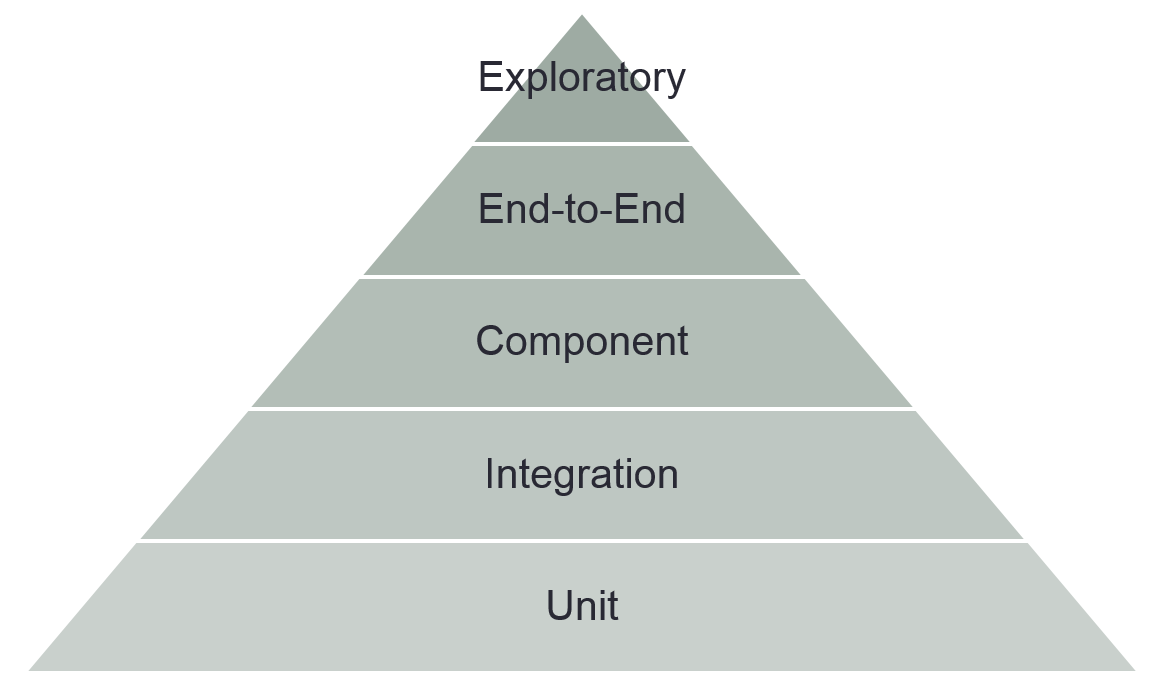
\includegraphics[width=0.7\textwidth]{./Images/FowlerPyramide.PNG}
    \caption{Test Pyramide von Martin Fowler}
    \label{fig:PyramideFowler}
\end{figure}
\subsubsection{Teststrategie von Google}
Die Teststrategie von Google ist keine Strategie explizit für Microservices, sondern eine generelle Teststrategie für die Produkte von Google. Dabei teilt Google seine einzelnen Tests sehr abstrakt und grob in drei Kategorien ein. Auch Google stellt seine Strategie mithilfe einer Pyramide dar, siehe Abbildung 3. Aus dieser Pyramide lassen sich die drei einzelnen Tests ablesen und zwar: 'Small Test', 'Medium Test' und 'Large Test'.

Ähnlich wie bei Fowler spielt auch hier die Position der Ebene eine Rolle. Je weiter unten sich eine Ebene befindet, umso mehr Test sollen davon ausgeführt werden. Das heißt von den Small Tests sollen die meisten durchgeführt werden. Zusätzlich gilt, je weiter unten die Ebene ist, umso isolierter sind die Tests und umso geringer sind die Ausführungsgeschwindigkeiten. Mit jeder Ebene mit der man nach oben geht, soll das Vertrauen in die Anwendung erhöht werden. Wie beim Ansatz von Fowler sollen auch hier die einzelnen Tests kurz in einer Auflistung erläutert werden \cite{whittaker2012google}.

\begin{itemize}
\item \textbf{Small Tests:} Wie der Name schon verrät sind hiermit die kleinsten Tests gemeint, welche sehr isoliert stattfinden sollen. Dazu sollen sie eine sehr geringe Ausführungsgeschwindigkeit haben, die im Millisekundenbereich liegen. Mit Small Tests sollen einzelne Funktion und Module getestet werden \cite{whittaker2012google}.
\item \textbf{Medium Tests:} Mit den Medium Tests sollen sogenannte Nachbar-Funktionen getestet werden. Darunter versteht Google ein Submodul von Funktionen, welche sich nacheinander und/oder gegenseitig aufrufen. Diese Tests sind nicht so schnell wie Small Tests. Die Ausführungsgeschwindigkeit soll dabei aber geringer sein als eine Sekunde. Dazu sind die Tests nicht so isoliert wie Small Tests und können auch externe Komponenten verwenden, die auf dieser Ebene nicht mehr durch ein Mock ersetzt werden sollen \cite{whittaker2012google}.
\item \textbf{Large Tests:} Die Large Tests haben die Aufgabe die komplette Anwendung oder Submodule davon zu testen. Dabei wird keine konkrete Ausführungs-
geschwindigkeit vorgegeben, sondern ist nur mit 'so schnell wie möglich' definiert. Dazu soll auf dieser Ebene verstärkt auf reelle externe Komponenten zurückgegriffen werden und weniger Mocks eingesetzt werden, als es bei Medium Tests der Fall ist \cite{whittaker2012google}.
\end{itemize}
\begin{figure}[htbp]
  \centering
      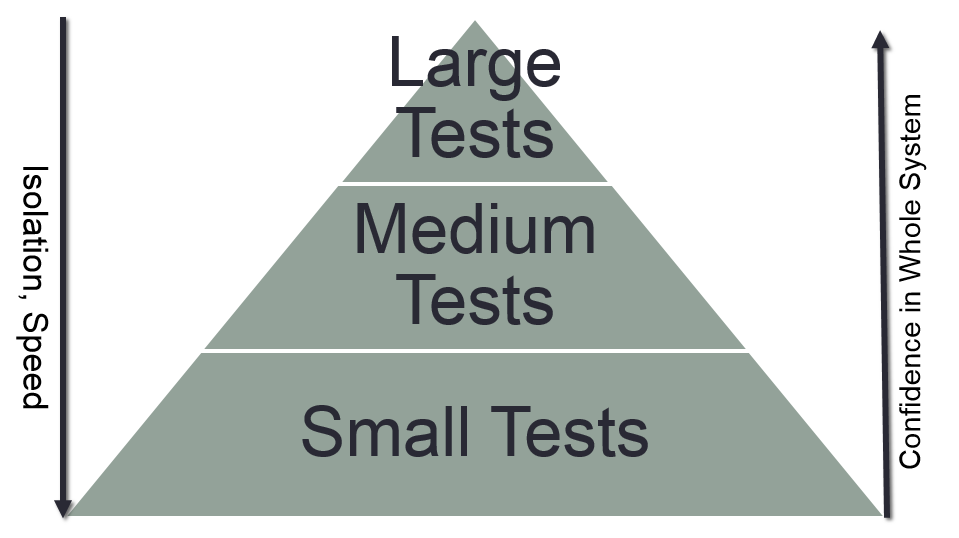
\includegraphics[width=0.7\textwidth]{./Images/GooglePyramide.PNG}
    \caption{Test Pyramide von Google}
    \label{fig:PyramideGoogle}
\end{figure}

\subsection{Fazit Grundprojekt}
Abschließend für das Grundprojekt kann man sagen, dass die grundlegende Arbeit erfolgt ist. Es wurde eine Testumgebung aufgebaut, mit der man experimentieren kann. Zudem erfolgte einer Einarbeitung in MARS und eine damit verbundene erste Analyse. Zudem wurden die Herausforderungen für das Testen von Microservice und speziell für MARS ausgearbeitet. Dazu wurden auch erste Systemtests mit dem Framework Selenium umgesetzt.

Für das Framework Selenium kann man das Fazit ziehen, dass Selenium eine schnelle Einarbeitung bietet und man recht schnell Testfälle via Selenium erstellen kann. Jedoch ist Selenium nicht gut geeignet für Anwendungen, an denen noch viel geändert wird. Besonders wenn man Elemente über den XPath sucht, zeigt Selenium große Schwächen. Da der XPath ein Pfad durch das HTML-Dokument wiedergibt, ist es dahingehend anfällig, wenn sich die Struktur des HTML-Dokuments ändert. Vereinfacht gesagt, wenn ein neues Element hinzu kommt oder entfernt wird und sich die Struktur des Dokuments ändert, kann sich auch der XPath zum gesuchten Element ändern. Wenn Selenium das Element unter dem angegeben XPath nicht findet, wirft es eine Exception und der Test schlägt fehl. In diesem Fall ist man gezwungen manuell zu prüfen, ob das Element wirklich nicht vorhanden ist oder ob sich nur der XPath geändert hat. Da man ursprünglich mit Selenium automatische Testabläufe haben möchte, ist dies sehr problematisch, da jedes manuelles Eingreifen dem widerspricht. Auf Grundlage dieses Ergebnis sollte eine Suche nach alternative Techniken für die Systemtests bzw. GUI-Test erfolgen.

Mit den bisherigen Testfällen werden circa 50\% der Microservices aufgerufen werden. Dies ist für die erste Testreihe ein durchaus guter Wert. Die Frage, die sich hier stellt, ist, wie man die weiteren Services abdecken kann ohne die Simulation zu starten. Dazu kommt auch noch die Frage, ob es wirklich sinnvoll ist, die Testabdeckung nach Abdeckung der Microservices zu definieren. Ergänzend dazu steht zu diesem Zeitpunkt noch nicht fest, wie die einzelne Abdeckung der Services aussieht. Dazu muss eine genauere Einarbeit in die Services stattfinden, um diese Frage zu beantworten.

Zudem erfolgte im Grundprojekt eine Recherche zum Thema Teststrategien für Microservices statt. Die vorgestellten Konzepte von Fowler und Google bieten interessante Möglichkeiten für eine Teststrategie bei Microservices. Da es zunächst nur eine Recherche stattfand, müssen noch weitere Untersuchungen folgen, um die jeweiligen Konzepte näher analysieren zu können und bewerten zu können. 

\section{Ausblick Hauptprojekt}
Im Hauptprojekt soll die bisherige Forschungsarbeit an MARS fortgesetzt werden. Dazu sollen zwei weitere Aspekte in die bisherige Forschung mit einbezogen werden. Zum einen soll ein Testkonzept für MARS entwickelt werden und zum anderen sollen die Integrationstests näher untersucht werden.

\subsection{Entwicklung eines Gesamtkonzeptes}
Im Hauptprojekt soll einerseits die Thematik der Teststrategie behandelt werden. Dabei ist auch der Plan für MARS eine Teststrategie zu entwickeln. Bevor die Teststrategie entwickelt werden kann, muss zunächst grundsätzliche Arbeit geleistet werden. Dafür sollen die beiden Ansätze, welche im Grundprojekt recherchiert wurden sind, miteinander verglichen werden, indem beide auf MARS angewendet werden. Beide Ansätze sind theoretisch angelegt und geben kaum Hinweise darauf, wie die einzelnen Tests in der Praxis, also mit welchen Werkzeugen und Technologien, umgesetzt werden sollen. Um dieses Problem zu lösen, soll auf bestehende Arbeiten aus dem Bereich Testen von Webservices und Service Oriented Architecure zurückgegriffen werden. Wie weiter oben schon erläutert, gibt es dort ähnliche Herausforderungen. Aus diesen Ergebnissen heraus soll eine passende Teststrategie für MARS entworfen werden. Dabei soll es auch um eine praktische Umsetzung gehen, wie man die einzelnen Tests umsetzen kann. 

\subsection{Integrationstests}
Neben der Entwicklung des Testkonzeptes für MARS wird ein weiterer Schwerpunkt auf die Integrationstest gesetzt. Dieser Schwerpunkt lässt sich nicht ohne weiteres von der Teststrategie trennen. Jedoch soll im Hauptprojekt ein besonderer Schwerpunkt auf diesem Aspekt gelegt werden. Aufgrund der Architektur ist das Zusammenspiel der einzelnen Services sehr entscheidend. Fehler in einem Service können sich schnell auf die gesamte Anwendung auswirken. Dahingehend ist es wichtig, die Services intensiv zu testen, damit die Services weiterhin gemeinsam funktionieren. Wie oben in den Herausforderungen schon formuliert, müssen diese Tests auch ein schnelles Feedback geben, damit weiterhin der Vorteil des schnellen Austausch von Services besteht. 

Es gibt viele verschiedene Technologien mit dem die Integrationstest durchgeführt werden können. Daher wird es eine Aufgabe in meinem Hauptprojekt sein, die verschiedenen Technologien zu sichten, zu analysieren und abschließend zu bewerten. Dabei sollen die einzelnen Technologien auch untereinander bewertet werden.

Um die Technologien für die Integrationstest bewerten zu können, müssen aber zunächst die Anforderungen definiert werden. Dementsprechend muss geklärt werden, was man genau von der Technologie erwartet. Dazu können noch weitere Anforderungen definiert werden, wie z.B. der Implementierungsaufwand, die Zugänglichkeit (Lizenz, etc.), Erweiterbarkeit und ob die Technologie noch weiter gepflegt wird.

In diesem Zusammenhang sollte auch die Frage geklärt werden, welche Rolle Docker dabei spielen kann. Docker wird bei MARS sehr verstärkt eingesetzt und bietet durchaus viele Anwendungsmöglichkeiten. Dahingehend sollte schon geprüft werden, ob Docker in diesem Kontext sinnvoll verwendet werden kann.

Die einzelnen Technologien sollen jedoch nicht nur auf dem Papier verglichen werden, sondern sie sollen auch in die Praxis umgesetzt werden. Dafür soll wieder in enger Zusammenarbeit mit dem MARS Projekt abgesprochen werden, an welchen Stellen die Integrationstests durchgeführt werden sollen.

Nach dem Praxiseinsatz werden die Technologien, wie oben schon beschrieben, analysiert und bewertet. Dabei werden selbstverständlich auch die vorher aufgestellten Anforderung mit einbezogen. Als Ergebnis für diesen Abschnitt soll fest stehen, wie und mit welcher Technologie man am besten die Integrationstests bei MARS durchführen kann.

Neben dem Aspekt der Technologien stellen sich auch hier Fragen hinsichtlich der Architektur bei MARS. In diesem Kontext sollte man untersuchen, ob es sinnvoll wäre enger gekoppelte Services als einen Service zu betrachten. Im SOA-Umfeld gibt es diesen Ansatz bereits und man spricht in dem Falle von einer Komposition. Zu Überlegen ist dabei, ob dies überhaupt von der Microservice-Architektur erlaubt wäre oder ob dies den Konventionen der Architektur widersprechen würde. Denn in den Definitionen von Microservice gibt es keine Anmerkungen zu Kompositionen. Des Weiteren stellt sich die Frage, ob es als Tester sinnvoll wäre enger gekoppelte Services als einen zu betrachten, um ggf. den Testprozess zu beschleunigen und somit ein schnelleres Feedback zu bekommen. Damit Änderungen schneller in den produktiven Code übergeben werden können. Untersucht werden müsste zusätzlich, was dies für die Integrationstest bedeutet. 

Da Integrationstests häufig sehr aufwendig sind und teilweise von der Ausführ-ungsgeschwindigkeit auch recht langsam sind, stellt sich hier die Frage, wie der Aufwand der Tests den Ablauf des Testen beeinflusst. Detailliert betrachtet heißt das, ob der Aufwand den Ablauf bestimmt, also sollten Tests mit geringen Aufwand als erstes oder als letztes ausgeführt werden. In dem Zuge stellt sich ebenso die Frage, wie der Aufwand die Häufigkeit der Tests bestimmt. Sollten Tests mit größeren Aufwand seltener durchgeführt werden und wenn ja, wie seltener.

\section{Fazit}
Wie im Fazit zum Grundprojekt schon beschrieben, legte das Grundprojekt ein wichtiges Fundament für die weitere Arbeiten im Hauptprojekt und in der Master-Arbeit. Die vorgestellten Arbeitspakete im Hauptprojekt, wie die Erarbeitung einer Teststrategie und der damit verbundene Fokus auf die Integrationstest, können ohne diese grundlegende Arbeit nicht durchgeführt werden.

Auf Grund der Verlagerung der Komplexität in die Infrastruktur bekommen die Integrationstest eine besondere Bedeutung. Wie im vorherigen Kapitel 4 'Ausblick Hauptprojekt' schon beschrieben, sollen die Integrationstest im Hauptprojekt einen Schwerpunkt bilden. Besonders hier gibt es viele offene Fragestellungen, die untersucht werden sollten. Dabei geht es sowohl um die generelle Technik, also wie erstellt man die Integrationstests und was soll getestet werden. Dazu soll auch untersucht werden, welche Technologien sich am besten dafür eignen. Es wird aber auch darum gehen, welchen Einfluss die Architektur auf die Testfälle hat. Testet man die Integration von allen Services untereinander oder nur von denen, welche eng gekoppelt sind? Dies sind nur eine Auswahl der vorhandenen Fragestellungen, welche intensiver im Hauptprojekt untersucht werden sollen.

Mit den Ansätzen von Martin Fowler und Google stehen zwei sehr interessante Ansätze zur Verfügung. Bei Martin Fowler ist vor allem die Definition der Integrationstests interessant. Bei seinem Ansatz testet der Anwender nur, ob der Service mit seinen eigenen externen Komponenten funktioniert. In seiner Theorie soll jedoch nicht getestet werden, ob die Services untereinander korrekt zusammenarbeiten. Er überspringt diesen Punkt, indem sein Ansatz vorsieht, dass als nächstes das komplette System getestet werden soll. Auch der Ansatz von Google ist vielversprechend interessant zu werden. Gerade hier wird sich zeigen, ob die Einteilung der Tests in der Praxis funktionieren. 

\bibliographystyle{alpha}
\bibliography{BIB_HSEM}

\end{document}